\documentclass[12pt,a4paper,openany]{article}
\usepackage{lmodern}
\usepackage{xcolor}
\input{../includesLaTeX/couleurs.tex}

\usepackage[utf8]{inputenc} \usepackage[T1]{fontenc}
\usepackage[francais]{babel}
\usepackage[top=1.7cm, bottom=1.7cm, left=1.7cm, right=1.7cm]{geometry}
\usepackage{verbatim}
\usepackage[urlbordercolor={1 1 1}, linkbordercolor={1 1 1}, linkcolor=vert1, urlcolor=bleu, colorlinks=true]{hyperref}
\usepackage{tikz} %Vectoriel
\usepackage{listings}
\usepackage{fancyhdr}
\usepackage{multido}
\usepackage{float}
\usepackage{amssymb}

\newcommand{\titre}{Dossier de spécifications des besoins logiciels}

\newcommand{\pole}{}
\newcommand{\sigle}{}

\newcommand{\semestre}{4}

\input{../includesLaTeX/listings.tex}
\input{../includesLaTeX/l2/docsProjet2.tex}
\input{../includesLaTeX/remarquesExempleAttention.tex}
\input{../includesLaTeX/polices.tex}
\makeatletter
\def\thickhrulefill{\leavevmode \leaders \hrule height 1ex \hfill \kern \z@}

\newlength{\sectiontitleindent}
\newlength{\subsectiontitleindent}
\newlength{\subsubsectiontitleindent}
\setlength{\sectiontitleindent}{-1cm}
\setlength{\subsectiontitleindent}{-.5cm}
\setlength{\subsubsectiontitleindent}{-.25cm}

\renewcommand{\section}{%
	\@startsection%
	{section}%
	{1}%
	{\sectiontitleindent}%
	{-3.5ex plus -1ex minus -.2ex}%
	{2.3ex plus.2ex}%
	{\sectionfont\Large}
}
\renewcommand{\subsection}{%
	\@startsection%
	{subsection}%
	{2}%
	{\subsectiontitleindent}%
	{-3.5ex plus -1ex minus -.2ex}%
	{2.3ex plus.2ex}%
	{\sectionfont\large}
}

\renewcommand{\subsubsection}{%
	\@startsection%
	{subsubsection}%
	{3}%
	{\subsubsectiontitleindent}%
	{-3.5ex plus -1ex minus -.2ex}%
	{2.3ex plus.2ex}%
	{\sectionfont\normalsize}
}

\makeatother

\newcommand{\lien}[1]{
 $\vartriangleright$ \url{#1}
 }

\newcommand{\pfp}{\texttt{pfp}}

\newcommand{\ifp}{\texttt{if}}
\newcommand{\elsep}{\texttt{else}}

\makeatother
\includeonly {
}
\begin{document}
	\setcounter{tocdepth}{2}
	\setcounter{secnumdepth}{3}
	\maketitle
	\tableofcontents
	\newpage
	\section{Introduction}
		\subsection{But du document}
	Le but de ce document est de lister toutes les fonctionnalités du futur logiciel et de son contexte d’utilisation (utilisateurs, autres composantes,
	matériel,  etc.).
		\subsection{Contexte de l'application}
		Cette application sera développé par Antoine de \bsc{Roquemaurel} et Fabrice \bsc{Valleix} dans le cadre du projet logiciel du 
		4\ieme{} semestre de l'année scolaire 2012--2013 de la L2 Informatique de l'université Toulouse III -- Paul Sabatier.
	
	\section{Description globale} 
	Le logiciel sera un jeu de Boggle$^{\tiny\textregistered}$ basé sur un dictionnaire en langue Française.

	Le jeu prend la forme d'une grille carrée, la taille étant donné par l'utilisateur. Dans chaque case de la grille est présente une lettre, au
	commencement du jeu, un compte à rebours de trois minutes est lancé, durant ces trois minutes le joueur doit chercher le plus de mots pouvant être
	formés à partir de lettre adjacentes du plateau, les mots doivent être de plus de 3 lettres et être présent dans le dictionnaire afin d'être
	acceptés.
	\subsection{Environnement}
		Le logiciel pourra être utilisé sur un ordinateur classique, sous GNU/Linux, aucun matériel externe ne sera nécessaire au bon fonctionnement du
		programme, de même le serveur d'interface graphique \texttt{X} ne sera pas utile, en effet le programme fonctionnera en mode texte ou semi graphique.
	\subsection{Profil des utilisateurs}
		Le logiciel possédera un unique profil d'utilisateur.
		\begin{description}
			\item[Le joueur] Il veut faire une partie de Boggle pour s'amuser ou passer le temps. L'ordinateur génère une grille de Boggle puis le
				joueur cherche des mots pendant 3 minutes en essayant de faire le plus de points possible. 
		\end{description}

	\section{Spécifications générales}
	\subsection{Description des services attendus}
	Les services attendus de l'application sont au nombres de deux.
		\begin{description}
			\item[Résoudre une grille par l'ordinateur] L'application doit être capable de résoudre une grille de Boggle, ceci peut importe la taille de
				la grille.
			\item[Effectuer une partie]  Et enfin, l'utilisateur devra pouvoir effectuer une partie de Boggle.
		\end{description}
	\subsection{Description générale des fonctions}
	Les fonctions sont réparties en deux catégories: celle qui seront utilisés pour la résolution d'une grille et celle indispensable pour effectuer
	une partie de Boggle.
	\subsubsection{Effectuer une partie de Boggle}
		\begin{description}
				\item[Génération d'une grille] L'application doit pouvoir générer une grille de Boggle, celle-ci devra être adaptée à la langue Française, en
				effet les lettres auront des probabilités d'apparaître en fonction de leur utilisation en Français, ceci afin d'éviter les grilles où
				l'utilisateur ne peut rien faire.
				
				Cette génération se fera en fonction de la taille de la grille fournie par l'utilisateur, cette taille doit être comprise entre 2 et 15.
				\item[Lancer le compte à rebours] Au départ de la partie, un compte à rebours de trois minutes doit être lancé. À la fin des trois
					minutes, l'utilisateur ne peut plus proposer de nouveau mot.
				\item[Proposition d'un mot] L'utilisateur peut proposer un mot, l'ordinateur l'accepte ou le refuse en fonction des critères suivants
					qui doivent tous être respectés:
					\begin{itemize}
						\item Présent dans la langue Française
						\item Longueur du mot supérieur ou égal à 3
						\item Suite de lettre dans la grille
						\item Mot non déjà utilisé
					\end{itemize}
				\item[Calcul du nombre de points obtenus] À la fin d'une partie, l'application doit afficher le nombre de points du joueur, et le
					nombre de points qu'il aurait pus faire s'il avait découvert l'intégralité des mots présents dans la grille, plus un mot est long
					plus il rapporte de points. Les points sont calculés ainsi:
					\begin{itemize}
						\item 3 et 4 lettres : 1 point
						\item 5 lettres : 2 points
						\item 6 lettres : 3 points
						\item 7 lettres : 5 points
						\item 8 lettres et plus : 11 points
					\end{itemize}
				\item[Possibilité de mettre fin au compte à rebours] L'utilisateur à la possibilité de terminer la partie avant que le
					compte à rebours arrive à zéro. Il peut vouloir mettre fin au compte à rebours parce qu'il pense avoir trouver
					tous les mots de la grille par exemple.
		\end{description}
	\subsubsection{Résoudre une grille de Boggle}
		\begin{description}
			\item[Résoudre une grille par l'ordinateur] 
				L'ordinateur doit pouvoir afficher la solution de la grille, c'est-à-dire une fois la partie finie l'ordinateur affiche tous les mots
				que l'utilisateur n'a pas trouvé.
			\item[Demande d'aide pour une lettre donnée] Pour une lettre donné, l'application doit afficher la longueur du mot le plus long qui
				commence par les lettres sélectionnées.
			\item[Affichage de la solution] 
				Afin d'afficher la solution l'application utilisera son résolveur. Il résout la grille et afficher ensuite tous les mots qui sont
				présent dans la grille avec les point correspondants.
		\end{description}
		\begin{figure}[H]
			\centering
			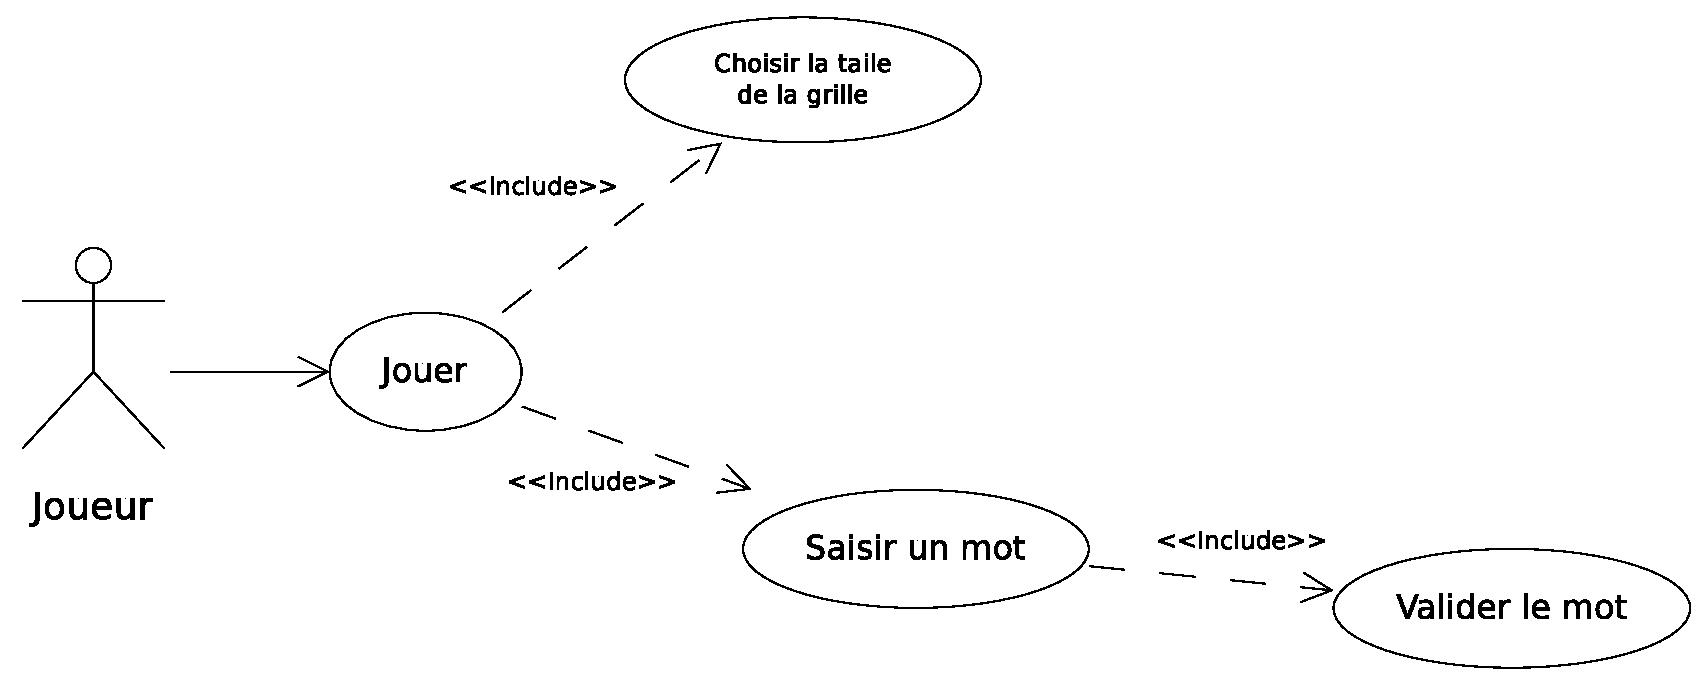
\includegraphics[width=15cm]{usecase.eps}
			\caption{Diagramme de cas d'utilisations}
		\end{figure}

	\section{Exigences opérationnelles} 
	\subsection{Modes de fonctionnement}
	Le logiciel disposera de deux modes de fonctionnements différents :
	\begin{itemize}
		\item Le mode texte
		\item Le mode pseudo graphique
	\end{itemize}
	Ces deux modes seront choisis en fonction des arguments du programme, par défaut l'application sera lancée avec le mode pseudo graphique.
	\subsection{Capacités}
	L'utilisateur doit fournir une taille de grille comprise entre 2 et 15.
	\subsection{Performances}
	Le temps de génération d'une grille et l'affichage de la solution seront fonctions de la taille fournie par l'utilisateur. Cependant dans le pire
	des cas, l'application ne devra pas mettre plus de 30 secondes à générer la grille et à fournir la solution.

	\section{Scénarios d'utilisations}
	\subsection{Scénario d'utilisation nominal}
	Voici un exemple de scénario possible dans son utilisation nominale.
		\begin{enumerate}
			\item Le système \textbf{demande la taille} de la grille de Boggle à l'utilisateur
			\item L'utilisateur \textbf{fournis la taille} de la grille 
			\item Le système \textbf{génère} la grille
			\item Le système lance un \textbf{compte à rebours} de 3 minutes
			\item L'utilisateur \textbf{propose} un mot
			\item Le système \textbf{accepte} le mot
			\item L'utilisateur \textbf{propose} un mot
			\item Le système \textbf{accepte} le mot
			\item L'utilisateur \textbf{propose} un mot
			\item Le système \textbf{refuse }le mot
			\item L'utilisateur \textbf{propose} un mot
			\item Le système \textbf{refuse} le mot
			\item Le \textbf{compte à rebours} arrive à 0
			\item Le système affiche le \textbf{nombre de points} obtenus
			\item Le système affiche la \textbf{solution}
		\end{enumerate}

		Un scénario alternatif pourrait apparaître aux étapes 5, 7, 9 et 11 l'utilisateur termine la partie, à ce moment là il se retrouverai automatiquement à
		l'étape 13.
	\subsection{Scénarios d'erreurs}
		À l'étape numéro 1 si l'utilisateur ne fournis pas un nombre entier compris entre 2 et 15, le système affiche un message d'erreur
			et relance l'étape numéro 1.
	
\end{document}

